\documentclass[UTF-8,openright]{ctexbook}

\begin{document}

%\title{清华园第四年}
%\author{张丹阳}
%\date{}
%\maketitle

\begin{titlepage}
	\centering
	\linespread{1.2}
	\vspace*{1cm}
	{\zihao{-0} \textbf{清华园第四年}\par}
	\vspace{0.5cm}
	{\zihao{-1} \textbf{——清华园怪谈集}\par}
	\vfill
	\begin{table}[!hb]
		\LARGE
		\centering
		\begin{tabular}{rc}
			作者: &	张丹阳 \\
			取材: &	程思源 \\
			&			张丹阳
		\end{tabular}
		\vspace{1cm}
	\end{table}
\end{titlepage}

\pagestyle{headings}

\pagenumbering{Roman}

\tableofcontents
\newpage

\pagenumbering{arabic}

\chapter{序章}

眨眼间我在清华园已度过了三年。
三年我吃过了园子里11个食堂,出入过4个图书馆,踏遍了6个教学楼,还借着阿甘跑步的时候跑遍了各种各样的小角落,自以为已对清华园非常熟悉了解。
然而,第四年,我却惊讶地发现,园子里还有这么多地方,我未曾踏足……

\vfill

\paragraph{记事}
2020年由于突发的疫情,在家里困了一个学期,6月份终于允许毕业生返校。
笔者毕业后就要去其他学校读博了,因此这本来是能够留在园子里的最后一个学期,只是如今仅剩下寥寥的数周了。
此番离去,之后回来的机会便少了许多。为了能够多留下些回忆,笔者约了朋友C君再在最后离校前逛一逛清华园。
晚上走在人迹罕至的小路上,就会有一种微妙的紧张与刺激感,于是便和C君聊起了魑魅魍魉、月黑风高的事情,谈笑间产生了杜撰些怪谈的想法。
笔者文笔枯燥乏力,实在缺乏表现力,本来只当个玩笑,但终于还是决定写下来,权做四年清华生活的纪念。
此间故事,皆为杜撰;怪力乱神,洵有其缘;茶余闲谈,供君一笑耳。

% 简要提纲
% 
% 1. 素材
%    * 荷塘南面,西湖西北,小山上,月黑杀人夜,风高放火天,零零阁
%    * 荷塘仿若小提琴声的荷香,荷仙的歌声,荷塘月色
%    * 装满水的西湖,服务看不见的客人
%    * 荷塘东侧的小山
%    * 夜晚的工字厅,门口的灯,冥府之门
%    * 苏世民书院后的凉风
%    * 二教的地下室,不开放自习,旧人体实验室
%    * 大礼堂后的小径,限时开放,大礼堂的地下室


\chapter{零零阁}

在荷塘南面,西湖北面,有一座小山。西边的山头上,有一座高大的阁子,唤作零零阁。%据说是以前“零零字班”的校友捐建的,因此得名。
1970年,适逢清华园学制由6年改为5年,两个年级的学生在同一年毕业。
当时校内习惯以毕业年份来作为届号,故早一年入学的称为“零字班”,晚一年入学的便称为“零零字班”。
这座阁子,便是由零零字班的校友捐建的。
阁子有两层,有着高高的螺旋台阶,矗立在山顶上,是这一范围内最高的建筑物,可以一览原来的皇家园林的秀美景观。

\begin{figure}[!b]
	\centering
	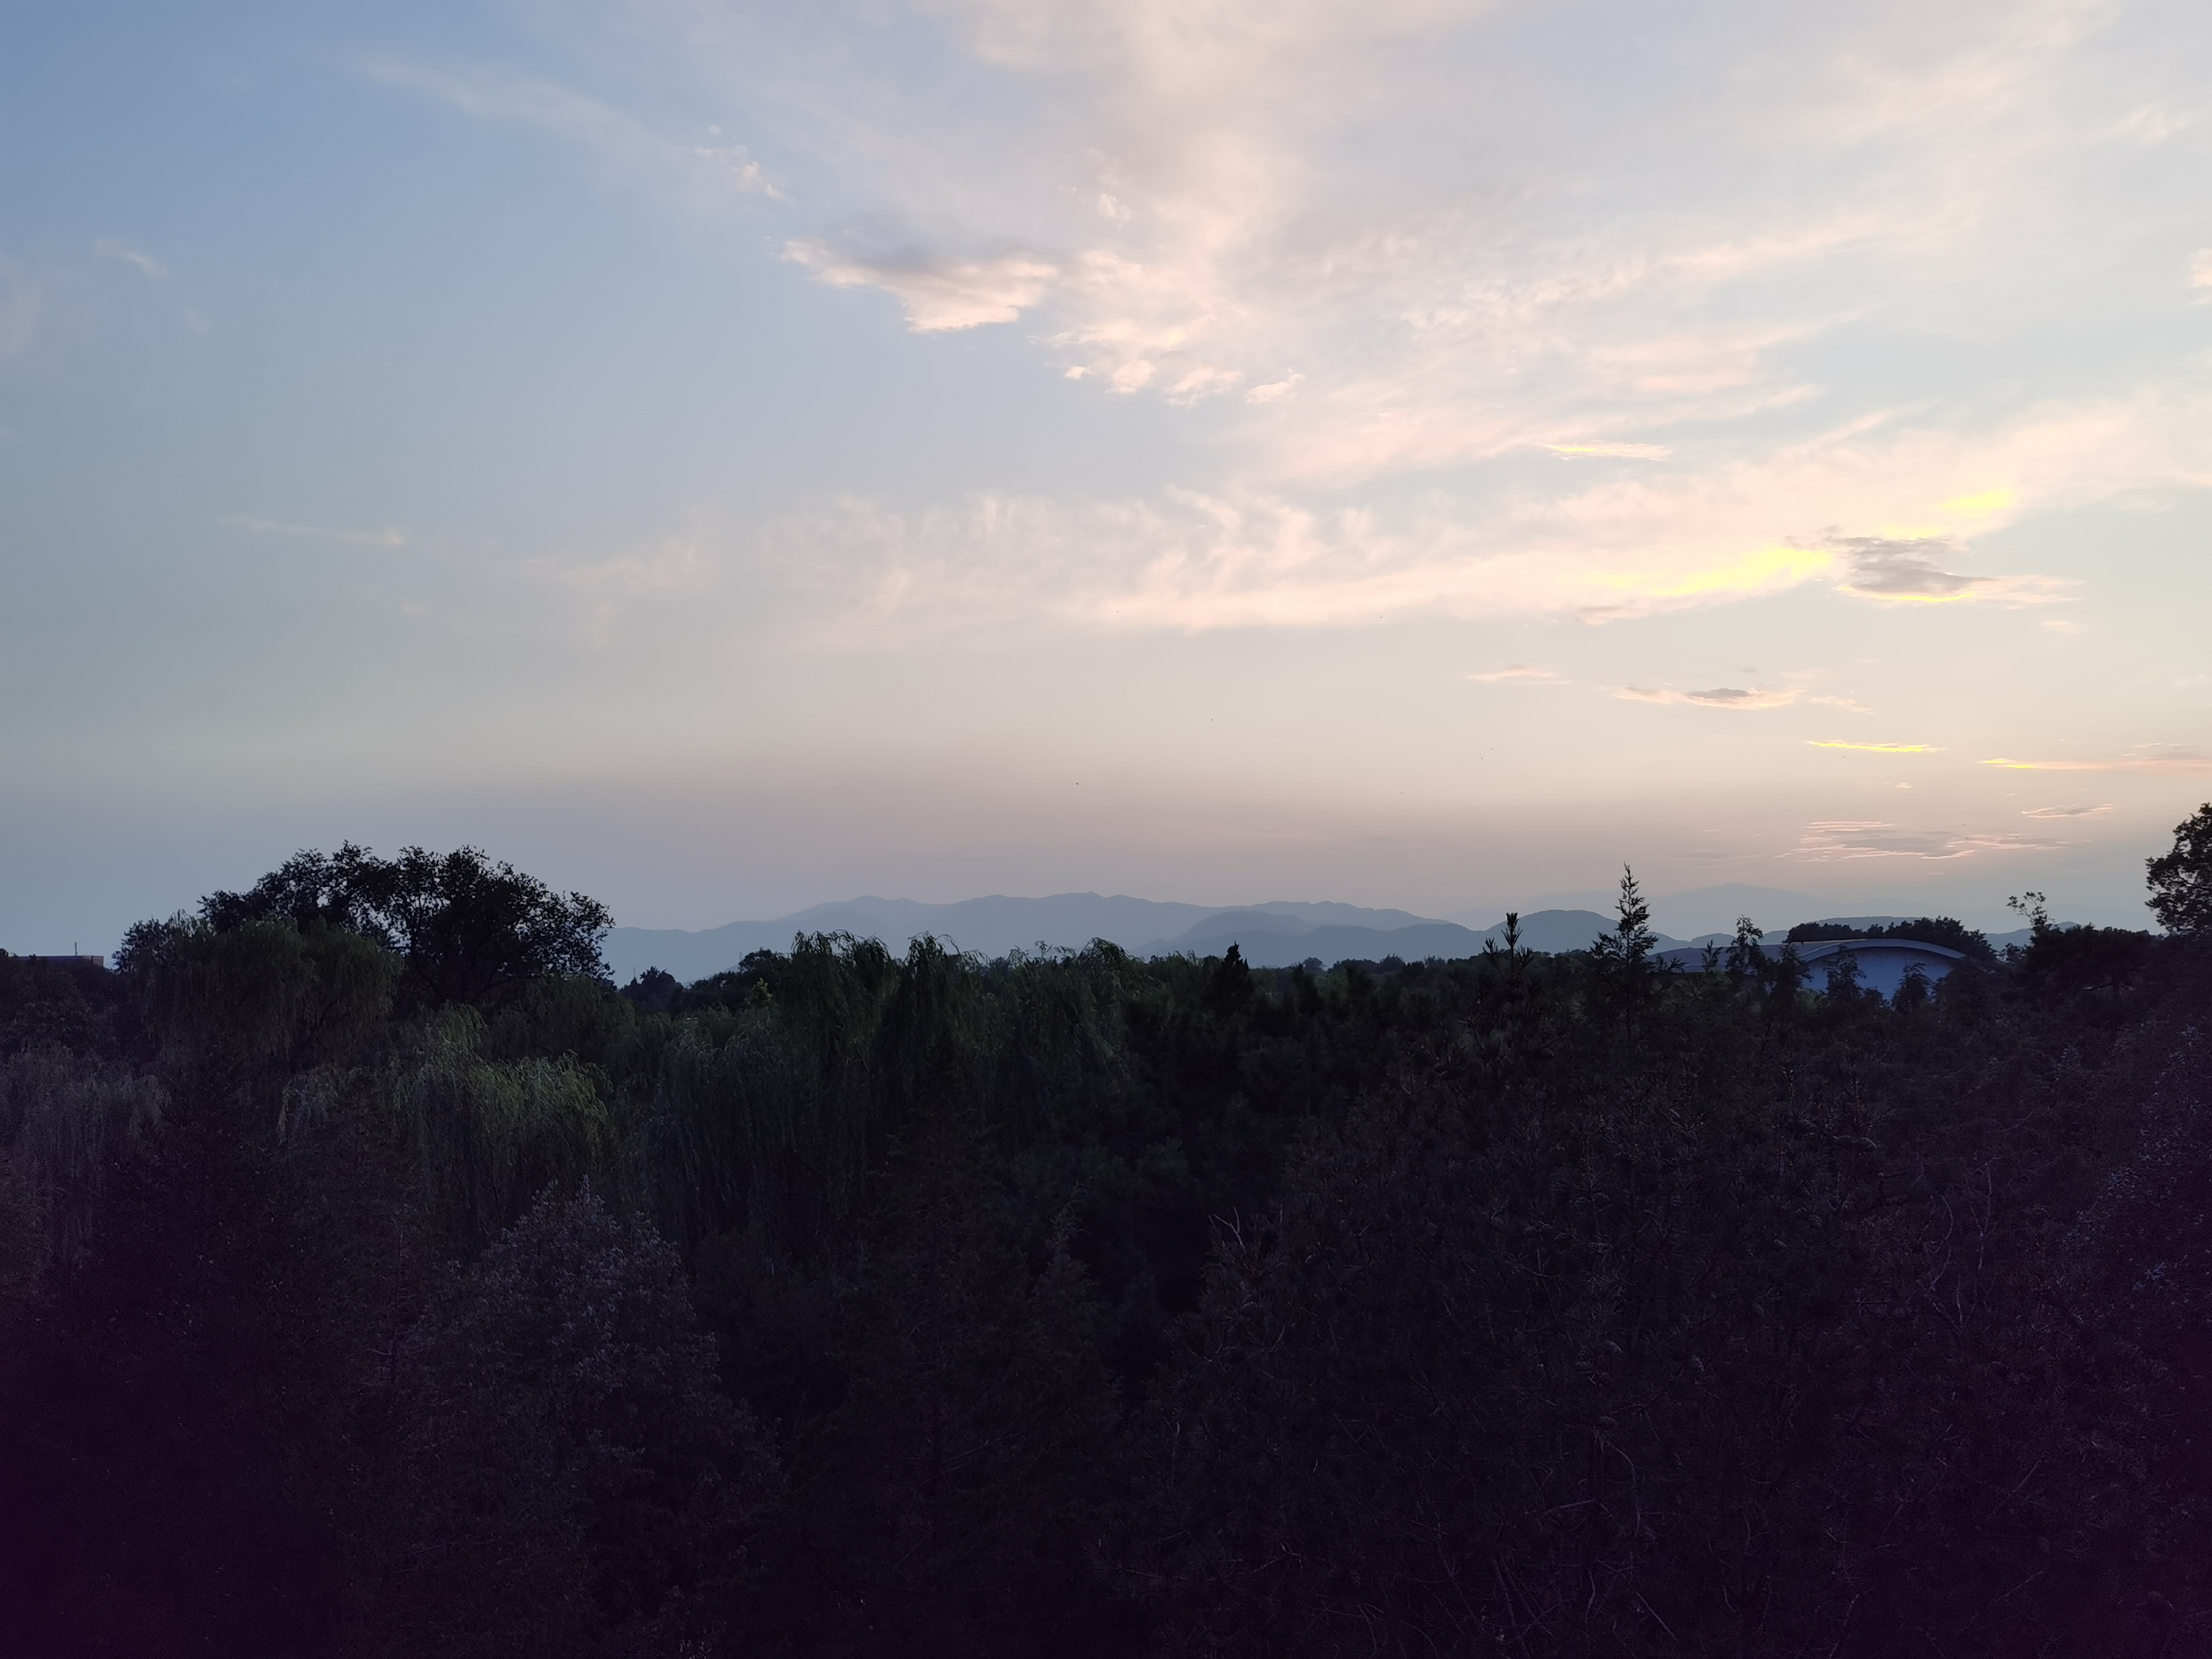
\includegraphics[width=\linewidth]{figures/零零阁暮望西山.jpg}
	从零零阁上远望西山。
\end{figure}

之前我与C君曾在阳光长跑时到过这个亭子。
当时跑得随性,只记得路过西湖附近,发现山上隐约有个亭子,便寻得路登了上去。穿过树丛,一座高大的亭子便豁然闯入眼帘。
我们正跑得气喘吁吁,然而登上二层后,阵阵凉风袭来,不胜清爽。
视野也陡然开阔。悠然东望,能从翠绿掩映中寻得六教深红的一角;极目向西,则甚至望得到远方巍巍西山:一时竟有种“一览众山小”的豪迈感,仿佛胸怀也随之变得更豁达了。
我们都对当时的场面印象深刻。于是C君提议,今日再登一次零零阁。

然而我们都已不记得这阁子的具体位置了,只大致记得应该是在荷塘旁靠近西湖的地方,于是我们便直奔荷塘而来。
荷塘北岸一马平川,自不可能有什么山巅的阁子。而湖心岛转过一遍,也没有发现符合当时印象的双层亭阁。
于是我们向荷塘南岸寻来。

荷塘这里靠近生活区,平时晚上就有许多人来这里散步、活动,因此相比园子里其他地方,有着浓浓的市井气息,仿佛城市里的公园一般。
然而晚上出来散步的人都聚集在荷塘北岸以及湖心岛的西北角,东面和南面的人烟便十分稀少,沿岸行走的话,仅间或能看到一两个默默垂钓的人。
我们沿荷塘东岸向南,至莲桥再向西。一过莲桥,就察觉这里人气已淡了许多。
太阳已经落山,又是阴天,浓云蔽月,再添上南岸茂密的树林,这时走在幽黑的林荫小径上,一阵凉风吹过,竟觉得有一些阴冷。
越向里走树木就越发茂密,光线也越来越暗,小径就仿佛没有出口的黑洞般,一直走不到尽头。这时我看到旁边有一条曲折延伸到山上密林中的小路。
微风吹过,我在这盛夏时节也不禁微微打了个寒颤,然后指着拐出去的小路说:“那亭子应该是在山顶上,我们一直沿着湖岸走要走到什么时候,不如往这里上去找一找。”C君亦以为然,于是我们便向山上走去。

\begin{figure}[!h]
	\centering
	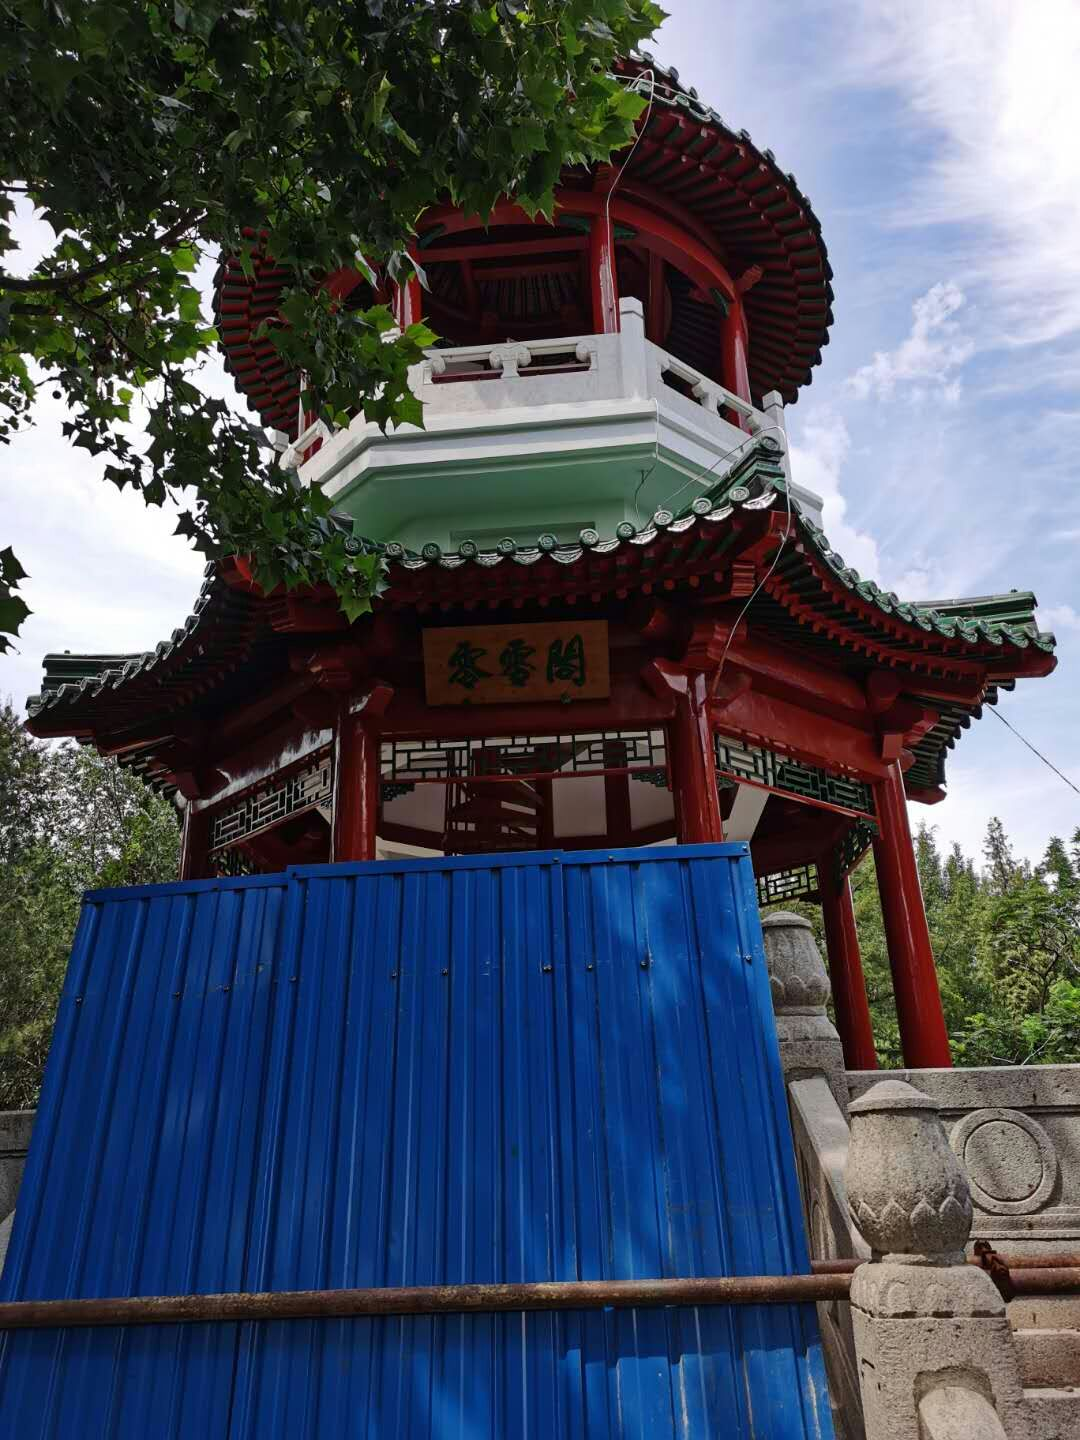
\includegraphics[width=\linewidth]{figures/零零阁.jpg}
	零零阁
\end{figure}

上山的小路坑坑洼洼的,许多铺路的石块都缺失了,表面还散布着细碎的石子,给人久未维护的感觉。
靠近山顶,树林稍稍稀疏了些,能够看到天上的阴云,也能看到前方朦胧的建筑,零零阁就在眼前了。
我们喜出望外,急忙沿着山路跑到了尽头,来到了心心念念的零零阁前,却惊讶地发现山路被围挡折断,亭子已整个被包围在其中,显然是正在翻修,无法再上去一瞰清华。大失所望之际,我们也只好再折返下山去。
这时一阵风穿过树林,发出尖锐的啸声,我们俩不禁又打了个哆嗦,不觉间已加快了下山的脚步。

就要走出湖边的小道时,迎面走来了一个满身酒气的人。
小径狭窄,几乎容不下他踉跄的步伐,我们只好赶紧闪到路边草坪上,让他先行过去。
兴许是刚刚赴完局,打算饭后找个清静少人的地方散散步,消消食,醒醒酒,随后便回家去,所以他也不顾夜色已深,便晃悠悠地走进了林荫小道,向荷塘南边走去。
素不相识,他的事,自然与我们无关,因而我们出来后,找到自己的自行车,便匆匆离去了。
当晚无事。

然而三天后的中午,C君突然急匆匆地找到我,递给我一份当日的报纸。
我低头一看,已下子就被报纸上的一条消息吓到了:
“昨日北京市某大学校内小山上某施工地点附近发现一具无头男尸,死状凄惨,全身血液流失殆尽。
法医初步鉴定死亡时间为两天前凌晨时段。
目前案件正在进一步调查中。”
报上黑白的配图虽然有些模糊,但我还是立刻就认出,那正是零零阁所在的那座小山……

\vfill

\paragraph{记事}
6月23日傍晚,笔者约C君出来共游校园,途中C君提到想再上一次零零阁,于是二人往西湖与荷塘这边寻来。
寻觅良久,终于在荷塘南边的小山上找到了亭子,却发现亭子已被围起来翻修了,失望而归。


% TODO: 请Oran作跋

\end{document}
